\documentclass[auto-toc=false,babel=ngerman]{arbeitsblatt}
\usepackage[utf8]{inputenc}
\title{Extremalprobleme}

\SetupExSheets{totoc}

\begin{document}
\maketitle

%\begin{framed}
% \noindent Strategie zum Lösen von Extremalproblemen
% \begin{itemize}
%  \item[(1)] Welche Größe soll extremal werden?
%  \item[(2)] Einführen der Variablen $x$. (Weshalb kann die in (1) genannte Größe verschiedene Werte annehmen, wovon hängt diese Größe ab?)
%  \item[(3)] Bestimmen der Zielfunktion. (Drücken Sie die Größe, die extremal werden soll, in $x$ aus. Beachten Sie die Definitionsmenge.)
%  \item[(4)] Untersuchen Sie die Zielfunktion auf Extremstellen.
%  \item[(5)] Formulieren Sie das Ergebnis. (Beachten Sie die Maßeinheiten.)
% \end{itemize}
%\end{framed}

\addsec{Aufgaben}

\begin{question}
  Wie groß ist die Summe, die man beim Addieren einer positiven Zahl und ihrer
  Kehrzahl erhält, mindestens?
\end{question}
\begin{solution}
  Die Summe einer Zahl und ihres Kehrwerts beträgt
  \begin{equation*}
    f(x) = x + \frac{1}{x} \qquad
    \definitionsmenge = \menge{x\in\reelle\vorausgesetzt x>0}
  \end{equation*}
  Der Extrempunkt wird wie üblich durch Ableiten und Nullsetzen gefunden:
  \begin{equation*}
    f'(x)  = 1 - \frac{1}{x^2} \quad
    f''(x) = \frac{2}{x^3}
  \end{equation*}
  Nullsetzen liefert die Lösung:
  \begin{gather*}
    0 = 1 - \frac{1}{x^2}
    \quad \Leftrightarrow \quad
    x^2 = 1
    \quad \Rightarrow \quad x = 1 \\
    f''(1) = 2 > 0
    \quad \Rightarrow\quad
    \text{Minimum bei $x=1$.}\\
    f(1) = 2
  \end{gather*}
  Die Summe einer Zahl und ihres Kehrwertes beträgt also mindestens $2$.
\end{solution}

\begin{question}
  Aus einem rechteckigen, \SI{10}{\centi\metre} langen und
  \SI{5}{\centi\metre} breiten Stück Pappe soll eine (oben offene) Schachtel
  mit möglichst großem Rauminhalt hergestellt werden.  Wie sind Länge, Breite
  und Höhe der Schachtel zu wählen?
\end{question}

\begin{solution}
  Skizze:
  \begin{center}
    \begin{tikzpicture}[scale=0.5]
      \draw (1,0) -- (9,0)  (1,5) -- (9,5) (0,1) -- (0,4) (10,1) -- (10,4);
      \draw[red]
        (0,0) -- (1,0) (9,0) -- (10,0)
        (0,5) -- (1,5) (9,5) -- (10,5)
        (0,0) -- (0,1) (0,4) -- (0,5)
        (10,0) -- (10,1) (10,4) -- (10,5);
      \draw
        (1,0) -- (1,1) -- (0,1)
        (0,4) -- (1,4) -- (1,5)
        (9,0) -- (9,1) -- (10,1)
        (9,5) -- (9,4) -- (10,4);
      \draw[red]
        (0.5,-0.3) node {$x$}
        (-0.3,0.5) node {$x$} ;
    \end{tikzpicture}
  \end{center}
  Als Hauptbedingung stellt man die Formel für das Volumen des Quaders auf:
  \[ V = abc \]
  Als Nebenbedingungen sind die vorgegebenen Maße des Kartons gegeben:
  \[  a = 10-2x \quad  b = 5-2x \quad c = x \]
  Einsetzen dieser Bedingungen ergibt die Zielfunktion:
  \begin{gather*}
    V(x)   = (10-2x)(5-2x)x = 4x^3 - 30x^2 + 50x \\
    V'(x)  = 12x^2-60x + 50 \quad
    V''(x) = 24x-60
  \end{gather*}
  Nullsetzen der ersten Ableitung liefert dann die Lösung:
  \[ 0 = 12x^2 -60x+50 \] Diese quadratische Gleichung hat die Lösungen $x_1
  \approx \num{3.943}$ und $x_2 \approx \num{1.057}$.  $x_1$ liefert eine
  negative Breite $b \approx \num{-2.887}$, also kann nur $x_2$ die gesuchte
  Lösung sein.  Damit ergeben sich die Werte $a \approx
  \SI{7.887}{\centi\metre}$, $b \approx \SI{2.887}{\centi\metre}$ und $c
  \approx \SI{1.057}{\centi\metre}$.
\end{solution}

\begin{question}
  Längs einer Hauswand soll ein rechteckiges Gartengrundstück so abgesteckt
  werden, dass zum Einzäunen der drei offenen Seiten eine Rolle mit
  \SI{20}{\metre} Maschendraht ausreicht.  Bei welchen Abmessungen wird das
  Grundstück am größten?
\end{question}
\begin{solution}
  Die Hauptbedingung ist die zu maximierende Fläche des Grundstücks:
  \[ A = ab \]
  Die Nebenbedingung ist durch die Länge des Zauns vorgegeben:
  \[ 20 = a+2b \quad\Leftrightarrow\quad a =20-2b \]
  Als Zielfunktion ergibt sich damit
  \begin{gather*}
    A(b)   = (20-2b)b = -2b^2+20b \\
    A'(b)  = -4b+20 \quad
    A''(b) = -4
  \end{gather*}
  Nullsetzen liefert nun die Lösung:
  \[
    0 = -4b+20 \quad \Leftrightarrow \quad
    b = 5 \quad\Rightarrow\quad
    a = 10
  \]
  Mit einer Breite von \SI{5}{\metre} und einer Länge von \SI{10}{\metre} ist
  der Flächeninhalt mit \SI{50}{\metre\squared} am größten.
\end{solution}

\begin{question}
  Welches Rechteck mit dem Umfang \SI{30}{\centi\metre} hat die kürzeste
  Diagonale?  (Hinweis: Bei dem gesuchten Rechteck hat das Quadrat über der
  Diagonalen minimalen Flächeninhalt.)
\end{question}

\begin{solution}
  Als Hauptbedingung benötigt man einen Zusammenhang zwischen Diagonale und
  Umfang, der sich mit dem Satz des Pythagoras aufstellen lässt.
  \[ d^2 = a^2+b^2 \]
  Als Nebenbedingung ist die Länge des Umfangs vorgegeben:
  \[
    30 = 2a+2b \quad \Leftrightarrow \quad b =15-a
  \]
  Setzt man das in die Hauptbedingung ein, kann man eine Zielfunktion
  aufstellen:
  \[ f(a) = d^2 = a^2 + (15-a)^2 \]
  Anstatt die Funktion aud $d$ aufzulösen, macht man es sich einfacher, wenn
  man $d^2$ als $f(a)$ setzt.  Wenn $d$ am kleinsten ist, dann ist auch $d^2$
  am kleinsten.
  \begin{gather*}
    f(a)   = 2a^2 - 30a + 225 \\
    f'(a)  = 4a-30 \qquad
    f''(a) = 4
  \end{gather*}
  Wie immer erhält man das Ergebnis, wenn man die erste Ableitung gleich $0$
  setzt.
  \begin{gather*}
    0 = 4a-30 \quad \Leftrightarrow \quad
    a = 7.5 \\
    \Rightarrow\quad b = 7.5
  \end{gather*}
  Das Quadrat mit der Seitenlänge \SI{7.5}{\centi\metre} hat die kürzeste
  Diagonale.
\end{solution}

\begin{question}
  Aus einem \SI{120}{\centi\metre} langen Draht soll das Kantenmodell eines
  Quaders hergestellt werden, bei dem eine Kante dreimal so lang ist wie eine
  andere und der Rauminhalt möglichst groß ist.
\end{question}
\begin{solution}
  Die Hauptbedingung ist das Volumen des Quaders:
  \[ V = abc \]
  Es sind zwei Nebenbedingungen vorgegeben.  Zum einen soll eine Kante dreimal
  so lang sein wie eine andere, $c = 3a$, und zum zweiten stehen
  \SI{120}{\centi\metre} für alle Kanten zur Verfügung:
  \[
    120 = 4(a+b+c) = 16a + 4b \quad\Leftrightarrow\quad
    b = 30-4a
  \]
  Einsetzen in die Hauptbedingung liefert die Zielfunktion:
  \begin{gather*}
    V(a)   = a(30-4a)3a = -12a^3 +90a^2 \\
    V'(a)  = -36a^2+180a \qquad 
    V''(a) = -72a+180
  \end{gather*}
  Die erste Ableitung muss $0$ gesetzt werden, um das Maximum zu finden:
  \begin{gather*}
    0 = -36a^2+180a = -36a(a-5) \\
    a_1 = 0 \qquad a_2 = 5
  \end{gather*}
  Für $a=0$ erhält man ein Minimum, ($V(0)=0, V''(0)=180$), also ist $a=5$ die
  gesuchte Lösung: $a = 5$, $b = 10$ und $c = 15$, jeweils in
  \si{\centi\metre}.  Das maximale Volumen ist  $V =
  \SI{750}{\cubic\centi\metre}$.
\end{solution}

\begin{question}
  Welche quadratische Säule mit der Oberfläche \SI{150}{\deci\metre\squared}
  hat den größten Rauminhalt?  Wie groß ist dieser?
\end{question}
\begin{solution}
  Die Hauptbedingung ist das Volumen der quadratischen Säule:
  \[ V = a^2h \]
  Als Nebenbedingung ist vorgegeben, dass die Oberfläche
  \SI{150}{\deci\metre\squared} betragen soll:
  \begin{gather*}
    150 = 2a^2 + 4ah \quad\Leftrightarrow\quad
    h = \frac{75}{2a} - \frac{a}{2}
  \end{gather*}
  damit ergibt sich für die Zielfunktion
  \begin{gather*}
    V(a)   = a^2\left(\frac{75}{2a} - \frac{a}{2}\right)
           = \frac{75}{2}a - \frac{a^3}{2} \\
    V'(a)  = \frac{75}{2} - \frac{3a^2}{2} \qquad
    V''(a) = -3a
  \end{gather*}
  Nullsetzen der ersten Ableitung liefert das Maximum:
  \begin{gather*}
    0 = \frac{75}{2} - \frac{3a^2}{2} \qquad\Leftrightarrow\qquad
    a^2 = 25 \\
    a = 5
  \end{gather*}
  Das negative Ergebnis $a=-5$ ist nur eine Scheinlösung, ein negative
  Kantenlänge ist nicht möglich.  Die Lösung ist also $h = 5$ mit $V = 125$.
  Damit hat der Würfel mit der Kantenlänge \SI{5}{\centi\metre}
  \SI{125}{\centi\metre\cubed} den größten Rauminhalt.
\end{solution}

\begin{question}
  Eine Holzkugel mit dem Radius $r=\SI{4}{\centi\metre}$ soll so abgeschliffen
  werden, dass ein Zylinder mit möglichst großem Rauminhalt entsteht.  Wie
  groß sind der Grundkreisradius und die Höhe des Zylinders?  Welchen
  Rauminhalt hat er?
\end{question}
\begin{solution}
  Skizze:
  \begin{center}
    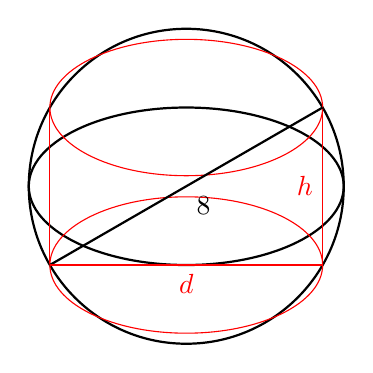
\begin{tikzpicture}[scale=0.5]
      \draw[thick] (0,0) circle (4cm);
      \draw[thick] (0,0) ellipse (4cm and 2cm);
      \draw[red] (0,2) ellipse (3.4641016cm and 1.7320508cm);
      \draw[red] (0,-2) ellipse (3.4641016cm and 1.7320508cm);
      \draw[red] (330:4cm) --node[left] {$h$} (30:4cm);
      \draw[red] (210:4cm) -- (150:4cm);
      \draw[thick] (210:4cm) --node[below right] {$8$} (30:4cm);
      \draw[red] (210:4cm) --node[below] {$d$} (330:4cm);
    \end{tikzpicture}
  \end{center}
  Die Hauptbedingung ist das Volumen des Zylinders \[ V = \pi r^2h \quad. \]
  Der Durchmesser und die Höhe des Zylinders bilden mit dem Durchmesser der
  Kugel als Hypotenuse ein rechtwinkliges Dreieick.  Als Nebenbedingung ist
  der Radius der Kugel vorgegeben.  Damit erhält man
  \begin{gather*}
    64 = d^2 + h^2 = 4r^2+h^2 \quad\Leftrightarrow\quad
    r^2 = 16 - \frac{h^2}{4} \quad.
  \end{gather*}
  Einsetzen in die Hauptbedingung liefert die Zielfunktion.
  \begin{gather*}
    V(h)   = \pi\left(16-\frac{h^2}{4}\right)h 
           = 16\pi h - \frac{\pi h^3}{4} \\
    V'(h)  = 16\pi - \frac{3\pi h^2}{4} \qquad
    V''(h) = -\frac{3\pi h}{2} < 0 \text{ da } h>0
  \end{gather*}
  Nullsetzen der ersten Ableitung:
  \begin{gather*}
    0 = 16\pi - \frac{3\pi h^2}{4} \quad\Leftrightarrow\quad
    h^2 = \frac{64}{3} \\
    h = \frac{8\sqrt{3}}{3} \approx \num{4.62}
  \end{gather*}
  Damit erhält man für den Radius des Zylinders $r = \frac{4\sqrt{6}}{3}
  \approx \num{3.27} $ und für das Volumen $V \approx \num{154.8}$.
  Der mit \SI{154.8}{\centi\metre\cubed} größte Zylinder hat den Radius
  \SI{3.27}{\centi\metre} und die Höhe \SI{4.62}{\centi\metre}.
\end{solution}

\begin{question}
  Einem gleichschenkligen Dreieck mit der Grundseite $c=\SI{12}{\centi\metre}$
  und der Schenkellänge $a=b=\SI{18}{\centi\metre}$ ist ein Rechteck mit
  maximalem Flächeninhalt einzubeschreiben.
\end{question}
\begin{solution}
  Skizze:
  \begin{center}
    \begin{tikzpicture}[scale=.35]
      \tkzInit[xmin=-1,xmax=13,ymin=-1,ymax=18]
      \tkzClip
      \tkzDefPoints{0/0/A,12/0/B,3/0/X,3/12/X',9/0/X''',9/12/X''}
      \tkzInterCC[R](A,18cm)(B,18cm)\tkzGetPoints{C}{C'}
      \tkzDrawPolygon(A,B,C)
      \tkzDefPointBy[projection=onto A--B](C)\tkzGetPoint{Mab}
      \tkzDrawSegment(C,Mab)
      \tkzInterLL(A,C)(X,X')\tkzGetPoint{X'}
      \tkzInterLL(B,C)(X''',X'')\tkzGetPoint{X''}
      \tkzDrawPolygon[color=red](X,X',X'',X''')
      \tkzLabelSegment[right](B,C){$18$}
      \tkzLabelSegment[below](A,B){$12$}
      \tkzLabelSegment[right,pos=.6](Mab,C){$h$}
      \tkzLabelSegment[below,pos=.6,color=red](X',X''){$a$}
      \tkzLabelSegment[left,color=red](X'',X'''){$b$}
    \end{tikzpicture}
  \end{center}
  Die Hauptbedingung ist der Flächeninhalt des gesuchten Rechtecks:
  \[ A = ab \quad. \]
  Das gleichschenklige Dreieck hat nach dem Satz des Pythagoras eine Höhe von
  $h=12\sqrt{2}\approx\num{16.97}$.  Nach dem zweiten Strahlensatz gilt:
  \[ \frac{h}{6} = \frac{b}{6-\frac{a}{2}} \] Mit $h=12\sqrt{2}$ ergibt sich
  dann als Nebenbedingung
  \[ b = 12\sqrt{2}-\sqrt{2}a \quad. \]
  Einsetzen in die Hauptbedingung gibt die Zielfunktion:
  \begin{gather*}
    A(a)   = a(12\sqrt{2}-\sqrt{2}a) = 12\sqrt{2}a-\sqrt{2}a^2 \\
    A'(a)  = 12\sqrt{2}-2\sqrt{2}a \qquad
    A''(a) = -2\sqrt{2}
  \end{gather*}
  Nullsetzen der ersten Ableitung liefert die Lösung:
  \begin{gather*}
    0 = 12\sqrt{2}-2\sqrt{2}a \quad\Leftrightarrow\quad
    a = 6 \\
  \end{gather*}
  Damit ist $b = 6\sqrt{2} \approx \num{8.59}$ und $A = 36\sqrt{2} \approx
  \num{50.91}$.  Das Rechteck mit den Maßen
  $\SI{6}{\centi\metre}\times\SI{8.59}{\centi\metre}$ hat also mit
  \SI{50.91}{\centi\metre\squared} den größten Flächeninhalt.
\end{solution}

\begin{question}
  Eine Zündholzschachtel soll \SI{5}{\centi\metre} lang sein und
  \SI{45}{\centi\metre\cubed} Inhalt haben.  Bei welcher Breite und Höhe
  braucht man zur Herstellung am wenigsten Material?
\end{question}
\begin{solution}
  Der Materialverbrauch hängt von der Pberfläche ab, was also
  dieHauptbedingung ist:
  \[ O = 2(5b+5c+bc) \]
  Als Nebenbedingungen sind Länge und Volumen vorgegeben.
  \[
    45 = 5bc \quad\Leftrightarrow\quad
    9 = bc \quad\Leftrightarrow\quad
    c = \frac{9}{b}, b>0
  \]
  Damit ergibt sich für die Zielfunktion:
  \[ O(b) = 2(5b + \frac{45}{b} + 9) = 10b + \frac{90}{b} + 18 \quad. \]
  Ableiten und Nullsetzen liefert die gesuchte Lösung.
  \begin{gather*}
    O'(b) = 10 - \frac{90}{b^2} \qquad
    O''(b) = \frac{180}{b^3} > 0 \text{ da } b>0 \\
    0 = 10 - \frac{90}{b^2} \quad\Leftrightarrow\quad
    b^2 = 9 \quad\Rightarrow\quad
    b = 3
  \end{gather*}
  Am wenigsten Material wird bei einer Breite und Höhe von je
  \SI{3}{\centi\metre} benötigt.
\end{solution}

\begin{question}
  Laut Gebührenordnung der Post dürfen bei Briefen in Rollenform die Länge und
  der zweifache Grundkreisdurchmesser zusammen höchstens
  \SI{104}{\centi\metre} betragen.  Bei welcher Länge und welchem Durchmesser
  nimmt eine solche Briefrolle am meisten Raum in Anspruch?  Wieviel
  \si{\deci\metre\cubed} beträgt dann der Rauminhalt?
\end{question}
\begin{solution}
  Die Hauptbedingung ist das gesuchte maximale Volumen
  \[ V = \pi r^2h \]
  Als Nebenbedingung ist vorgegeben, dass die Summe aus zwei Durchmessern und
  der Länge nur \SI{104}{\centi\metre} betragen darf:
  \[ 104 = 4r+h \quad\Leftrightarrow\quad h = 104-4r \]
  Damit ergibt sich nun als Zielfunktion:
  \begin{gather*}
    V(r)   = \pi r^2(104-4r) = 104\pi r^2 -4\pi r^3 \\
    V'(r)  = 208\pi r - 12\pi r^2 \qquad
    V''(r) = 208\pi - 24\pi r
  \end{gather*}
  Nullsetzen der ersten Ableitung ergibt die gesuchte Lösung:
  \begin{gather*}
    0 = 208\pi r - 12\pi r^2 = r(52-3r) \\
    r_1 = 0 \qquad r_2 = \frac{52}{3} \approx \num{17.33}
  \end{gather*}
  Das Ergebnis $r_1=0$ ergibt ein Minimum, $V(0)=0$, die gesuchte Lösung ist
  logischerweise $r_2 \approx \num{17.33}$.
  \begin{gather*}
    \Rightarrow\quad d = \frac{104}{3} \approx \num{34.67} \\
    h = \frac{104}{3} \approx \num{34.67} \quad
    V \approx 32721
  \end{gather*}
  Bei einem Durchmesser und einer Länge von je \SI{34.67}{\centi\metre} hat
  die Briefrolle den maximalen Rauminhalt \SI{32.72}{\deci\metre\cubed}.
\end{solution}

\begin{question}
  Eine Elektronikfirma verkauft monatlich 5000 Stück eines Bauteils zum
  Stückpreis von \SI{25}{€}.  Eine Marktforschung hat ergeben, dass sich der
  monatliche Absatz immer dann um durchschnittlich 500~Stück erhöhen würde,
  wenn der Stückpreis um \SI{2}{€} gesenkt wird.  Welcher Stückpreis ist für
  die Firma am günstigsten?
\end{question}
\begin{solution}
  Am günstigsten ist, da wir von statischen Produktionskosten ausgehen müssen,
  wenn die Einnahmen maximal sind.  Dann ist die Hauptbedingung
  \[ E = sp \]
  wobei $E$ die Einnahmen in Euro sind, $s$ die verkaufte Stückzahl und $p$
  der Preis pro Stück in Euro.  Pro Preissenkung um einen Euro erhöht sich die
  Stückzahl um 250.  Als Nebenbedingung ergibt sich daraus
  \begin{gather*}
    s = 5000 + 250x \\
    p = 25-x \quad\Leftrightarrow\quad x = 25 -p \\
    s = 5000 + 250(25-p) = 11250 - 250p \quad.
  \end{gather*}
  Damit haben wir schließlich als Zielfunktion
  \[ E(p) = (11250 - 250p)p = 11250p - 250p^2 \quad. \]
  Ableiten und Nullsetzen liefert wie üblich die gesuchte Lösung.
  \begin{gather*}
    E'(p) = 11250 -500p \qquad  E''(p) = -500<0 \\
    0 = 11250 -500p \quad\Rightarrow
    p = 22.5
  \end{gather*}
  Am günstigsten ist also ein Stückpreis von
  \SI[round-mode=places,round-precision=2]{22.50}{€}.
\end{solution}

\addsec{Lösungen}
\printsolutions

\end{document}
